\documentclass[12pt, a4paper, openany]{book}
\usepackage{fstyle}

\graphicspath{ {./img/} }

\begin{document}
\title{Esami di Analisi Matematica}
\author{Fabio Ferrario}
\date{2022}
\maketitle
\tableofcontents

\chapter{Introduzione}
\section{Gli esami}
La professoressa Pini ha fornito, tramite E-Learning alcune prove d'esame degli anni precedenti:
\paragraph*{Primo Semestre}
\begin{tabular}{ |c|c|c|c| }
	\hline
	Esame         & Crocette   & Domande Aperte & Note \\
	\hline
	Febbraio 2019 &            &                &      \\
	Gennaio 2020  &            &                &      \\
	Febbraio 2020 & \checkmark &                &      \\
	Gennaio 2021  &            &                &      \\
	Febbraio 2021 & 7/8        &                &      \\
	Gennaio 2022  &            &                &      \\
	Febbraio 2022 &            &                &      \\
	\hline
\end{tabular}
\paragraph*{Secondo Semestre}
\begin{tabular}{ |c|c|c|c| }
	\hline
	Esame       & Crocette & Aperte & Note                                 \\
	\hline
	Giugno 2019 & 8/8      & 3/3    & Manca un pezzo della domanda $1ii$   \\
	Giugno 2020 & 7/8      & 2/4    &                                      \\
	Giugno 2021 & 6/8      & 0/3    &                                      \\
	Luglio 2019 & 8/8      & 0/2    & La domanda aperta 1 è da trascrivere \\
	Luglio 2020 & 8/8      & 2.5/3  &                                      \\
	Luglio 2021 & 5/7      & 1.9/2  &                                      \\
	\hline
\end{tabular}

\chapter{Esami Primo Semestre}
\section{Febbraio 2021}

\domanda{1}{Sia $a_n = \frac{n \ln (1- \frac{2}{n^3})}{n \sqrt[3]{n} - n^3}$. Allore, per $n \to +\infty$,
}
\risposta{$a_n \sim \frac{2}{n^5}$}
\spiegazione{
	$$
		a_n = \frac{n \ln(1-\frac{2}{n^3})}{n \sqrt[3]{n}-n^3} \rightarrow \frac{\frac{2}{n^2}}{n^3} \rightarrow \frac{2}{n^2} \cdot \frac{1}{n^3} = \frac{2}{n^5}
	$$
	Bisogna trovare una successione asintoticamente equivalente sia per il numeratore, che per il denominatore.
}
\domanda{2}{Sia $f:\R \to \R$ con $f'(0)=0,f''(x)=ln(e+x)$.Allora $f$ ha in $x=0$}
\risposta{Un punto di minimo Relativo}
\irrisolta

\domanda{3}{Sia $f:\R \to \R$ una funzione continua e dispari. Allora, $\int_{-3}^{4} f(x) dx$ è uguale a}
\risposta{$\int_{3}^{4} f(x) dx$}
\spiegazione{Una funzione dispari è una funzione che ha il grafico simmetrico rispetto all'origine, quindi ha $f(-a) = -f(a)$.
	L'integrale è l'area sottesa della funzione \emph{con il segno}, quindi in una $f(x)$ dispari $\int_{-a}^{a} f(x) dx = 0$ (Spiegazione negli appunti).
	Di conseguenza è intuibile che in questa funzione l'integrale da -3 a 3 si annulla, e rimane solo l'area da 3 a 4.}


\domanda{4}{La derivata della funzione $f(x) = \sqrt[3]{\frac{x^3}{2} +1}$ è}
\risposta{$\frac{x^2}{2\sqrt[3]{(\frac{x^3}{2}+1)^2}}$}
\spiegazione{
	La derivata di una funzione composta è: $f(g(x))' = f'(g(x))\cdot g'(x)$.
	Per quanto riguarda la radice, è meglio farla a mano trasformandola ($\sqrt[\alpha]{x^\beta} = x^\frac{\beta}{\alpha}$).
	Il resto sono calcoli Algebrici
}

\domanda{5}{la serie $\serie{1}{+\infty} \frac{1}{n^{(\alpha+1)/2}\ln^2n}$ }
\risposta{Converge sse $\alpha \geq 1$}
\spiegazione{Siccome $n^{...}$ si moltiplica al logaritmo, se fosse infinitesimo annullerebbe il denominatore rendendo la serie divergente a infinito.
	Quindi, l'esponente di alpha deve essere positivo, di conseguenza $\alpha \geq 1$}


\domanda{6}{La funzione $f(x) = \begin{cases}a \sin x - b^2  & -2 \leq x \leq 0 \\ 1-e^x &0<x\leq 3\end{cases}$ è derivabile in $x=0$ se e solo se:}
\risposta{$a=-1,b=0$}
\spiegazione{
	Una funzione è derivabile in un punto se è continua e se i limiti destro e sinistro della derivata in quel punto coincidono.
	\\Verificando la continuità, è banale che $b^2=0 \to b=0$.
	\\Verficiando i limiti della derivata invece:
	$ f(x) = a sinx \implies f'(x) = a cos(x)$, $\limite{x}{o^-} a cos(x) = a$.
	\\ $f(x) = 1 -e^x \implies f'(x) = -e^x$, $\limite{x}{o^+} -e^x = -1$.
	\\Di conseguenza, $a = -1$ per la derivabilità.
}


\domanda{7}{Quali tra questi insiemi è un intervallo?}
\risposta{$\{x \in \R: 2|x| \geq x^2\}$}
\spiegazione{}

\domanda{8}{Date le funzioni $f(x) = \ln(x), g(x)= x^3, h(x) = 2-x$, la funzione composta $(h \circ g \circ f)(x)$ è:}
\risposta{$2-\ln(x)$}
\spiegazione{$(h \circ g \circ f)(x) = h(g(f(x)))$}

\section{Febbraio 2022}
\domanda{O1}{$f(x) = \ln(x^3-1)$, $g(x) = |x|$, la funzione $(f \circ g)(x)$ è:}
\risposta{$ln(|x|^3-1)$}
\spiegazione{$(f\circ g)(x) = f(g(x))$}

\domanda{O2}{La funzione $f(x) = \begin{cases} 4\frac{e^{2x-1}}{x} & x<0 \\ x^2 + \frac{a}{2} & x\geq0\end{cases}$ ha in $x=0$ una discontinuità di prima specie sse:}
\risposta{$a\neq 16$}
\spiegazione{Una discontinuità di prima specie la si ha quando i limiti destro e sinistro di $x_0$ esistono finiti e non coincidono.
	\\$f(0) = \frac{a}{2}$, quindi basta mettere $a$ in modo che sia diverso dal limite destro.
		\\$\limite{x}{0^-} f(x) = \frac{0}{0}$, che è una forma di indecisione.
	Usando il limite notevole dell'esponenziale decido di  moltiplicare e dividere per $2x$:
	$ 4\frac{e^{2x-1}}{2x} \cdot \frac{2x}{x} = 4 \cdot 1 \cdot \frac{2x}{x} = 8$
	Di conseguenza $a\neq 16$.
}
\domanda{O3}{$f:\R \to \R$ derivabile e tale che $f(1)=4$ e $f'(1)=-2$. Se $g(x)= \ln(f^2(x)+1)$, allora $g'(1)$ vale:}

\risposta{$-\frac{16}{17}$}
\spiegazione{Si può trovare $g'(1)$ senza sapere $f$. Basta derivare $g(x)$ mantenendo $f(x)$ come se fosse un incognita:
	$g'(x)=\frac{1}{f^2(x)+1}\cdot 2f(x) \cdot f'(x) = \frac{2f(x) \cdot f'(x)}{f^2(x)+1}$
	Valuto $g'(1)$ sostituendo a $f(x)$ e $f'(x)$ le loro valutazioni in uno e trovo $g'(1)=-\frac{16}{17}$
}
\domanda{O4}{L'insieme $A=\{\frac{\ln n}{n},n=1,2,...\}$}
\risposta{Ha minimo 0}

\domanda{O5}{Una primitiva della funzione $f(x)=\frac{e^{2x}}{e^{2x}+1}$ è:}
\risposta{$\frac{\ln(e^{2x}+1)}{2}+7$}
\spiegazione{Si può notare che l'espressione $e^{2x}$ è ripetuta, si deduce quindi che è conveniente provare per sostituzione.
\\Pongo $y=e^{2x}$ e isolo la $x$: $x=\frac{\ln y}{2}$.
\\Ora derivo a sinistra e destra e "moltiplico" ripsettivamente per $dx$ e $dy$, quindi: $\ddx[x] = dx$
e $\ddx[\frac{\ln y}{2}] = \frac{1}{2} \cdot \ddx[\ln y] = \frac{1}{2y} dy$
\\Sostituisco con $y$ e $dy$ nella funzione originale:
$$\int \frac{\cancel{y}}{y+1} \cdot \frac{1}{2\cancel{y}} dy = \frac{1}{2} \int \frac{1}{y+1}dy$$
Sappiamo che $\int \frac{1}{y+1}dy = ln(y+1) +c$, quindi:
$$=  \frac{ln(y+1)}{2} +c \to \text{Sostituisco}\to \frac{\ln(e^{2x}+1)}{2}+c$$
}

\domanda{O6}{$\limite{n}{+\infty} n^2\sin(\frac{1}{n+n^2})$ vale}
\risposta{1}
\spiegazione{
	Sappiamo che per $x\to0, \sin(x)\sim x$, quindi:
	$\sim n^2\cdot \frac{1}{n+n^2}= \frac{n^2}{n+n^2} \sim \frac{n^2}{n^2} = 1$
}

\domanda{O7}{$f(x) = e^{3x-x^3}$ è monotona decrescente sse}
\risposta{$x\in(-\infty,-1] \vee x\in [1,+\infty)$}
\spiegazione{Per trovare la monotonia faccio la derivata
$f'(x)=e^{3x-x^3}(3-3x^2)$ e la pongo $\geq 0$
$e^{3x-x^3}\geq 0 \forall x$, $3-3x^2\geq 0 \to 3x^2-3\leq 0 \to x\leq \pm 1$
Quindi $x \geq 0$ tra $-1$ e $1$.

}

\domanda{O8}{La serie $\sum_{n=1}^{+\infty} \frac{5}{2n^{2-a}+4}$ converge sse }
\risposta{$a<1$}
\spiegazione{
	$\sim \frac{1}{n^{2-a}}$, perchè converga il denominatore deve avere esponente $>1$, quindi $a<1$.
}

\subsection{Domande Aperte}
\domandaaperta{1}{Sia $f:\R \to \R$ definita da $f(x)=(2-x^2)e^x$. Allora:}
\rispostaaperta{
	\paragraph*{Dominio} Tutto $\R$
	\paragraph*{Limiti} $\limite{x}{+\infty} = +\infty$
	\\$\limite{x}{-\infty} = \infty \cdot 0$, indecisione DA FARE
		\paragraph*{Asintoti} DA FARE (viene AOr $y=0$ per $x\to -\infty$ )
		\paragraph*{Derivata} $f'(x)=-2xe^x+e^x(2-x^2)=e^x(-x^2-2x+2)$
		\paragraph*{Monotonia} $f'(x)\geq 0 \to -x^2-2x+2\geq 0 \to x^2+2x-2 \leq 0$
		\\$x_{12} = \frac{-2\pm\sqrt{12}}{2}$ (Notare che alla prof viene $\pm\sqrt{3}-1$, che è equivalente)
	Dallo studio del segno risulta che la funzione è Monotona Crescente con $x\in [\frac{-2-\sqrt{12}}{2},\frac{-2+\sqrt{12}}{2}]$
	\paragraph*{Estremi} Dallo studio della mnonotonia notiamo che:
	\\$\frac{-2-\sqrt{12}}{2}$ è Minimo Relativo, dato che la funzione dopo va a meno infinito.
		\\$\frac{-2+\sqrt{12}}{2}$ è Massimo Assoluto, dato che dallo studio della monotonia notiamo che è la "punta" dell'unico intervallo in cui la funzione è crescente.
	\paragraph*{Derivata Seconda} $f''(x) = e^x(-x^2-2x+2)+(-2x-2)e^x = e^x(-x^2-4x)$
	\paragraph*{Concavità e Convessità} $f''(x)\geq 0 \to x^2+4x\leq 0 \to -4\leq x \leq 0$
	\\Dallo studio del segno risulta che la funzione è convessa in $x\in [-4,0]$
	\paragraph*{Mclaurin II ordine} $P(x)=2+2x$
	\paragraph*{Retta tangente al grafico} al punto $x=1$.
	\\Trovo $m=f'(1)= -e$, trovo $q=f(1) - f'(1) \cdot 1 = 2e$.
	\\La retta tangente al grafico al punto $x=1$ ha equazione: $y=-ex+2e$
}
\domandaaperta{2}{Data la serie $\serie{1}{+\infty} q^n$, dove $q\in \R$, la serie:}
\rispostaaperta{converge sse $q\in(-1,1)$, diverge sse $q\in[1,+\infty)$ ed è infefinita sse $q\in(-\infty,1]$}
\domandaaperta{2b}{Si consideri la serie $\serie{0}{+\infty} (\frac{2x}{x^2+1}^n$, con $x\in\R$)}
\rispostaaperta{La serie \emph{non converge} sse:
	\\$\frac{2x}{x^2+1}\geq 1 \to 2x\geq x^2+1$, $x_{12}= 1$
		\\è indeterminata sse: $\frac{2x}{x^2+1}\leq -1 \to x=-1$.
		\\per $x=-2$ la somma della serie vale: $\frac{5}{9}$}
\domandaaperta{3}{Data la funzione funzione $f(x)=x-\frac{\ln^2x}{x} : (0,+\infty) \to \R$:
	\begin{itemize}
		\item Si scrivano tutte le primitive
		\item Si determini, se esiste, la primitiva $\phi$ tale che $\phi(e) = 2\phi(1)$
		\item Si calcoli $\int_{e}^{e^2}f(x) dx$.
	\end{itemize}
}
\irrisolta

\chapter{Esami Secondo Semestre}

\section{Giugno 2019}
\subsection{Domande Chiuse}
\domanda{1}{La serie $\serie{1}{+\infty}(-1)^n sin(\frac{3}{n^2})$}
\risposta{Converge assolutamente}
\spiegazione{
	Siccome abbiamo sia $(-1)^n$, che una successione $\sin(a_n)$, sappiamo che questa serie è a \emph{segno variabile}.
	\\Usiamo quindi il criterio dell'assoluta convergenza.
	$$
		|\serie{1}{+\infty}(-1)^n sin(\frac{3}{n^2})| = |sin(\frac{3}{n^2})| \sim \frac{3}{n^2}
	$$
	la corrispondenza asintotica vale perchè l'argomento del seno è infinitesimale.
	La successione risultante è una serie armonica di grado $> 1$, quindi converge.
}
\domanda{2}{La Successione $a_n = \frac{\ln(2+n^3)-5\sqrt[]{n^2-n}+2^{-n^4+5n}}{5n+3\ln n - n \ln n}}$ per $n \to +\infty$ ha limite:
\risposta{$\limite{n}{+\infty} = 0$}
\spiegazione{
	Si trova una successione asintoticamente equivalente sia per numeratore, che per denominatore.
	$$ a_n \sim \frac{2^{-n^4}}{5n}$$
	Si noti che nel numeratore, $2^{-n^4 +5n}$ il $+5n$ è "sovrastato" da $-n^4$, quindi è ignorabile.
	\\Siccome al numeratore abbiamo un valore infinitesimo,($ = (\frac{1}{2})^{n^4}$), la successione tende a $0$
}

\domanda{3}{La funzione $f(x) = \frac{2x^3+4x}{2-x^2} + e^{-\frac{1}{x}}$, per $x\to +\infty$, ha asintoto obliquo di equazione:}
\risposta{$$y=-2x+1$$}
\spiegazione{
	Per trovare un asintoto obliquo bisogna trovare $m$ e $q$ che compongono la retta $y=mx +q$:
	\\$
	m=\limite{x}{+\infty}\frac{f(x)}{x}
	= \frac{\frac{2x^3+4x}{2-x^2} + e^{-\frac{1}{x}}}{x}
	= (\frac{2x^3+4x}{2-x^2} + e^{-\frac{1}{x}})\cdot \frac{1}{x}
	= \frac{2x^3+4x}{2x-x^3} + \frac{e^{-\frac{1}{x}}}{x}
	= \frac{\cancel{x}(2x^2+4)}{\cancel{x}(2-x^2)} + \frac{e^{-\frac{1}{x}}}{x}
	\sim \frac{2\cancel{x^2}}{-\cancel{x^2}} + \frac{e^{-\frac{1}{x}}}{x}
	= -2 + \frac{e^{-\frac{1}{x}}}{x}
	$. Siccome $\frac{e^{-\frac{1}{x}}}{x}$ tende a $0$, allora $m$ equivale a $-2$
		\\Adesso dobbiamo trovare $q$
		\\$
		q = \limite{x}{+\infty} [f(x) -mx]
		= \frac{2x^3+4x}{2-x^2} + e^{-\frac{1}{x}} +2x
		\sim \frac{2\cancel{x^3}}{-\cancel{x^2}} + e^{-\frac{1}{x}} +2x
		=\cancel{-2x} + e^{-\frac{1}{x}} \cancel{+2x} = e^{-\frac{1}{x}} = 1
	$
	\\Quindi, l'asintoto obliquo esiste e ha equazione $y=-2x+1$
}

\domanda{4}{Sia $f(x) = \sqrt{x^2 +2x +3}$. allora $f'(1)$ vale:}
\risposta{$\frac{2}{\sqrt{6}}$}
\spiegazione{
	Basti ricordarsi che:
	\\La derivata di una radice è: \derivata{\sqrt[\alpha]{x}}{\frac{1}{\alpha \sqrt[\alpha]{x}}}
	\\Questa funzione è una funzione composta ($f(x) = \sqrt{g(x)}$), quindi bisogna derivarla come tale: $f(g(x)) = f'(g(x)) \cdot g'(x)$.
	\\Una volta calcolata la derivata e semplificata fino a un punto "comodo", basta sostituire $x$ con 1.
}

\domanda{5}{L'insieme delle soluzioni della disequazione $e^x \sqrt[3]{x-1} \geq 1$ è del tipo}
\risposta{$(\alpha, +\infty)$ con $\alpha>1$}
\spiegazione{
	Ci si chiede l'intervallo dei valori di $x$ per cui la disequazione è sostanzialmente "corretta", quindi quando il termine sinistro è maggiore di 1.
	\\Se si prova un po per esclusione, si vede che per $x=0$ è "falsa" e rimane così anche per valori minori di 0.
	\\$x=1$ ci da 0, quindi deve essere per forza un valore maggiore di 1
}

\domanda{6}{la funzione $f(x) = \ln(x^2+2x+3)$ è monotona crescente se e solo se}
\risposta{$x\in (-1,+\infty)$}
\spiegazione{
	Per trovare se una funzione è \emph{monotona crescente} bisogna porre la derivata della funzione $\geq 0$.
	Il risultato è $x\geq -1$, che equivale a $x\in (-1,+\infty)$.
}
\domanda{7}{L'estremo inferiore della successione $\{a_n\}_{n\geq0}$, dove $a_n = 3^{n+(-1)^nn}$ è:}
\risposta{
	1
}
\spiegazione{
	Per vedere l'estremo inferiore di una successione bisognerebbe provare qualche valore di $n$ a partire dal più piccolo (in questo caso 0).
	Se il termine è infinitesimale, l'estremo inferiore si trova con il limite, altrimenti vedi il valore minore che trovi.
}
\domanda{8}{$\int_{\pi/2}^{\pi} x \sin x dx$ vale:}
\risposta{
	$\pi -1$
}
\spiegazione{
	Integro per parti, quindi abbiamo:
	\\$f(x) = x$ e quindi $f'(x) = 1$
		\\$g'(x)= \sin(x)$ e quindi $g(x) = -\cos(x)$
	\\Risolvo con la formula dell'\emph{integrazione per parti}:
	$$x (-\cos(x)) - \int 1(-\cos(x)) = -x\cos(x)+\sin(x) = \sin(x)-x\cos(x)$$
	Risolvo l'integrale per gli estremi dati:
	$F(\pi) = \pi$, $F(\pi/2)=1$.
	Quindi l'integrale dato vale $\pi -1$
}

\subsection{Domande Aperte}
\domandaaperta{1i}{Data la serie $\serie{1}{+\infty} (\frac{x^2+6}{5x})^n$, Si determino i valori di $x\in\R \backslash \{0\}$ per cui converge, e se ne calcoli la somma.}

\rispostaaperta{
	La serie è di tipo gemoetrico con ragione $q=\frac{x^2+6}{5x}$, e per convergere deve essere $|q|<1$.
	$$|\frac{x^2+6}{5x}| < 1 = \frac{x^2+6}{|5x|}<1$$
	Risolviamo quindi per $x<0$ e per $x>0$.
	\begin{equation*}
		\begin{cases}
			x>0 \\
			\frac{x^2+6}{5x} < 1 = \frac{x^2+6}{5x} -1 < 0 =\frac{x^2+6-5x}{5x} < 0
		\end{cases}
	\end{equation*}
	Siccome $5x > 0$ è valido sempre per $x>0$, risolviamo solo il numeratore e troviamo $2<x<5$
	\\Facendo la stessa cosa per $x<0$ (con il denominatore di $q$ invertito di segno) trovo  $-2<x<-3$
	Quindi, per i valori di x compresi tra $-2<x<-3$ e $2<x<3$ la somma della serie vale:

	$$
		S=\frac{1}{1-\frac{x^2+6}{5x}} - 1 =\frac{5x}{5x-x^2+6} - 1 = \frac{x^2+6}{5x-x^2-6}
	$$
	\nb{il "$-1$" va messo perchè la formula della serie geometrica si applica solo alle serie che partono da 0,
		quindi per le serie che partono da 1 la formula diventa $\frac{1}{1-q} - (q)^0$, ovvero si toglie il termine con $n=0$.
	}
}
\domandaaperta{1ii}{
Si studi la funzione $f(x)=\frac{(x+1)^2}{3x(2x-1)}$ (Limiti ai punti di frontiera del dominio, Eventuali asintoti, monotonia, grafico qualitativo. NON è richiesto lo studio della derivata seconda).
\\Si calcolino l'estremo superiore e l'estremo inferiore di $f$ relativamente all'intervallo $[1,+\infty)$, specificando se sono anche massimo e/o minimo su tale intervallo.
}
\rispostaaperta{
	\paragraph*{Dominio della funzione} $3x(2x-1)\neq 0 \to x\neq 0 \wedge x\neq \frac{1}{2}$, quindi
	la funzione è definita in $\R\backslash\{0,\frac{1}{2}\}$
	\paragraph*{Limiti agli estremi del dominio}
	$$\limite{x}{\pm\infty} f(x) = \frac{\infty}{\infty} \text{ Indecisione!}$$
	Riformulo quindi la funzione
	$$\limite{x}{\pm\infty} f(x) = \frac{x^2+1+2x}{6x^2-3x} \sim \frac{\cancel{x^2}}{6\cancel{x^2}} = \frac{1}{6}$$
	$$\limite{x}{0^+} f(x)= \frac{1}{0^+(-1)} = \frac{1}{0^-} = -\infty$$
	$$\limite{x}{0^-} f(x)= \frac{1}{0^-(-1)} = \frac{1}{0^+} = +\infty$$
	$$\limite{x}{\frac{1}{2}^+} = \frac{\frac{9}{4}}{\frac{3}{2}(0^+)} = \frac{\frac{9}{4}}{0^+} = +\infty $$
	$$\limite{x}{\frac{1}{2}^-} = \frac{\frac{9}{4}}{\frac{3}{2}(0^-)} = \frac{\frac{9}{4}}{0^-} = -\infty $$

	\paragraph*{Asintoti}
	Dai limiti, si deduce che:
	\begin{itemize}
		\item $\frac{1}{6}$ è Asintoto Orizzontale per $x\to \pm \infty$.
		\item $x=0,x=\frac{1}{2}$ sono Asintoti Verticali.
	\end{itemize}

	\paragraph*{Monotonia}
	Per calcolare la monotonia di una funzione bisogna verificare i punti in cui la derivata della funzione è maggiore o uguale a zero.
	faccio la \emph{derivata prima}
	$f(x) = \frac{(x+1)^2}{3x(2x-1)}$, quindi usando le formule base per le derivate ottengo:
	$$
		f'(x) = \frac{2(x+1)(3x(2x-1))-((12x-3)(x+1)^2)}{(3x(2x-1))^2}
	$$
	Risolvo alcuni calcoli aritmetici:
	$$
		= \frac{6x(x+1)(2x-1)-((12x-3)(x+1)^2)}{9x^2(2x-1)^2}
	$$
	Raccolgo $(x+1)$ nel numeratore:
	$$
		= \frac{(x+1)((6x(2x-1))-((12x-3)(x+1)))}{9x^2(2x-1)^2}
	$$
	Risolvo alcuni calcoli aritmetici:
	$$
		= \frac{(x+1)((12x^2-6x)-(12x^2+12x-3x+3))}{9x^2(2x-1)^2}
	$$
	$$
		=\frac{(x+1)(\cancel{12x^2}-6x-\cancel{12x^2}-12x+3x+3)}{9x^2(2x-1)^2}
	$$
	$$
		=\frac{(x+1)(-15x+3)}{9x^2(2x-1)^2}
	$$
	Raccolgo il 3 dal secondo membro del numeratore:
	$$
		=\frac{(x+1)3(-5x+1)}{9x^2(2x-1)^2}
	$$
	Finisco con un calcolo aritmetico:
	$$
		=\frac{(x+1)(-5x+1)}{3x^2(2x-1)^2}
	$$
	\subparagraph*{Pongo la derivata $\geq 0$}
	Per trovare gli intervalli in cui la funzione è crescente.
	$$
		\frac{(x+1)(-5x+1)}{3x^2(2x-1)^2} \geq 0
	$$
	Studio il segno dei 4 polinomi della derivata e li unisco:
	\\$x+1\geq 0 \to x\geq -1$,e $-5x+1\geq 0 \to x\leq \frac{1}{5}$ per il numeratore,
		\\ $3x^2>0 \to \forall x$,e $(2x-1)^2>0 \to \forall x$ per il denominatore.
		\\Unisco i risultati e ottengo:
		\\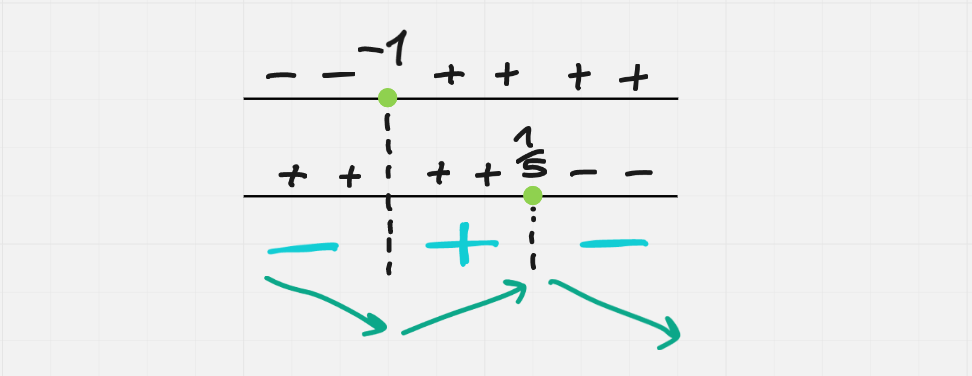
\includegraphics[width=\textwidth]{disequaz-giugno-2019.png}
		quindi $f'(x)\geq 0$ se e solo se $x\in [-1,0)\cup (0,\frac{1}{5}]$ (nota che zero è escluso perchè è punto di disconitinuità).
		\\In particolare, $x=-1$ è punto di minimo relativo, $x=\frac{1}{5}$ è punto di massimo relativo.

		\paragraph*{Grafico Qualitativo}
		Per tracciare il grafico, conosco i punti di discontinuità, i limiti e gli asintoti.
		\\Per comodità, trovo: $f(-1)=0$ e $f(\frac{1}{5})=-4$ e traccio il grafico:
	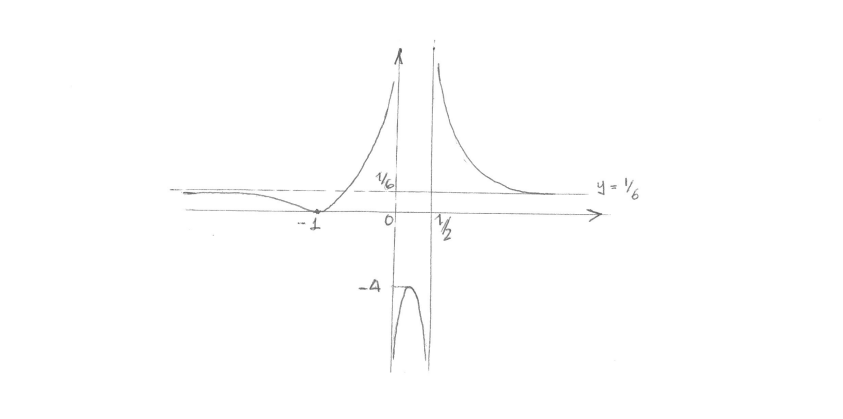
\includegraphics[width=\textwidth]{grafico-giugno-2019.png}
}
\domandaaperta{2}{
Si enunci il teorema di esistenza del limite per successioni monotone.
\\Data la successione:
$$
	a_n = \ln(n+1)-\ln n = \ln(\frac{n+1}{n}) \text{ con } n\geq 1
$$
\textbf{i.} si verifichi, utilizzando la definizione, che è monotona (crescente o decrescente?);
\\\textbf{ii.} si calcoli $\limite{n}{+\infty}(\ln(n+1)-\ln n)$
\\\textbf{iii.} si calcoli la somma della serie $\serie{1}{+\infty}(\ln(n+1)-\ln n)$
	}
	\rispostaaperta{
		\paragraph*{Teorema di esistenza del limite:}
		Se una successione è monotona crescente allora il limite esiste e coincide con l'estremo superiore della successione.
		\\Se invece è monotona decrescente allora il limite esiste e coincide con l'estremo inferiore della successione.
		\paragraph*{i}
		Si vuole dimostrare che la successione sia monotona (crescente o decrescente).
		\\Notiamo che la successione si può semplificare in: $a_n=\ln(1+\frac{1}{n})$, il che ci rende le cose molto più facili:
		\\intuitivamente notiamo che $a_{n+1}<a_n$, quindi:
		$$a_{n+1} = \ln(1+\frac{1}{n+1}) < ln(1+\frac{1}{n}) = a_n$$
		e, siccome $\frac{1}{n+1}<\frac{1}{n}$ e la funzione logaritmo è crescente ($\ln(n)<\ln(n+1)$)
		ne consegue che la serie $\{a_n\}$ è \emph{Monotona Decrescente}.
		\paragraph*{ii}
		$limite{n}{+\infty} a_n = \ln(1+\frac{1}{n}) = \ln(1) = 0$.
		\\Volendo si può dire anche che per un $x\to0$ il logaritmo di $(1+x)$ è asintotico ad $x$, in questo caso quindi sarebbe asintotico a $\frac{1}{n}$, ovvero 0.

		\paragraph*{iii}
		La serie $a_n$ è a termini positivi e $\ln(n+1) - \ln(n) \sim \frac{1}{n}$ (vedi sopra), pertanto è divergente ($+\infty$)s.
	}

	\section{Giugno 2020}
	\subsection{Domande Chiuse}
	\domanda{1}{La funzione $f:\R \to \R$ definita da $f(x)=\begin{cases}e^x & x>0 \\ x+2 & x\leq 0\end{cases}$ è}
	\risposta{Suriettiva ma non Iniettiva}
	\spiegazione{
		La funzione è \emph{suriettiva} perchè riempie tutto $\R$.
		Per controllarlo basta vedere i grafici dei due segmenti della funzione.
		\\Non è iniettiva invece perchè ci sono dei punti del codomino "raggiungibili" con due $x$ diverse.
		Per verificarlo basti vedere che nel grafico della funzione id due segmenti si accavallano su alcuni valori di $y$.
	}

	\domanda{2}{Siano $f(x) = e^{\sqrt{x}}$ e $g(x)= \ln(1+x)$. Allora $(g \circ f)$}
	\risposta{è definita per ogni $x\geq 0$}
	\spiegazione{$g\circ f = g(f(x)) = ln(1+e^{\sqrt{x}})$, quindi bisogna vedere dove è definita quella funzione.
	\\Sappiamo che l'argomento di una radice va posto maggiore o uguale a zero, e quello di un logaritmo va posto maggiore di 0}

	\domanda{3}{La somma della serie $\serie{1}{+\infty} e^{1-2n}$ vale}
	\risposta{$\frac{e}{e^2-1}$}
	\spiegazione{
		La serie si può riscrivere come:
		\\$\serie{1}{\infty} e^{1-2n} = e\sum (\frac{1}{e^2})^n$
			\\Essendo una serie geometrica con argomento minore del modulo di 1, si può risolvere con la formula risolutiva.
			Siccome però la serie parte da 1, bisogna togliere la somma con n=0 (moltiplicata per la costante $e$), quindi:
			\\$= e \frac{1}{1-\frac{1}{e^2}} -e = \frac{e}{1-\frac{1}{e^2}}-e
			= \frac{e}{\frac{e^2-1}{e^2}}-e
			= e\frac{e^2}{e^2-1}-e = \frac{e^3}{e^2-1}-e = \frac{e^3-e^3+e}{e^2-1}
			=\frac{e}{e^2-1}
		$
		\\nota che il $-e$ sarebbe $-e\cdot(q)0$
	}
	\domanda{4}{Sia $f:\R \to \R$ la funzione definita da $f(x) = \int_{1}^{x} t^2 e^{\sqrt[3]{t}} dt$. Allora:}
	\risposta{$f$ è Crescente}
	\irrisolta

	\domanda{5}{$\limite{n}{+\infty} \frac{n^2 \ln^3 n - n^3 \ln^2 n +4 \arctan n}{n^3 \ln^2 n - n^2 \ln^5 n- e^{-n^2}}$ vale:}
	\risposta{-1}
	\spiegazione{$\frac{n^2 \ln^3 n - n^3 \ln^2 n +4 \arctan n}{n^3 \ln^2 n - n^2 \ln^5 n- e^{-n^2}} \sim \frac{-n^3 \ln^2 n}{n^3 \ln^2 n} = -1$}

	\domanda{6}{Il massimo dell'insime $A = {\frac{2+(-1)^n}{2^n+(-1)^{n+1}}}$ è}
	\risposta{1}
	\spiegazione{per $n=2$ l'insieme vale 1, mentre per tutti gli altri valori di n è minore.}


	\domanda{7}{sia $f(x) = \arctan(\sqrt{x})$. Allora $f'(1)=$}
	\risposta{Nessuna delle precedenti ($\frac{1}{4}$)}
	\spiegazione{Trovo la derivata della funzione:
		\\$f'(x) = \frac{1}{1+x} \cdot \frac{1}{2\sqrt{x}} = \frac{1}{2\sqrt{x}(1+x)}$. La derivata vale in $x=1$:
		$f'(1) = \frac{1}{4}$}

	\domanda{8}{Sia $f$ definita e continua su [a,b]. Allora}
	\risposta{Assume il valore $\frac{f(a)+f(b)}{2}$}
	\spiegazione{Non ho trovato nessuna definizione che giustifichi questa cosa, ma da Telegram mi dicono:
		Se una funzione è continua in un intervallo ed ho $y_1 = f(a)$ e $y_2 = f(b)$ allora la funzione può assumere tutti i valori tra $y_1$ e $y_2$.
		$\frac{f(a)+f(b)}{2}$ se lo guardi nell'asse delle y è un valore compreso tra $f(a)$ e $f(b)$.
		\\Un'altra risposta corretta potrebbe essere: Assume tutti i valori tra $f(a)$ e $f(b)$.
	}

	\subsection{Domande Aperte}
	\domandaaperta{1}{
		Si determinino $a$ e $b$ affinchè la funzione:
		\begin{equation*}
			f(x)= \begin{cases}
				a\frac{\ln(x-1)}{x-2} +bx  & x>2             \\
				2x^2-2x+1                  & 0 \leq x \leq 2 \\
				a(x+1)+3\frac{e^{bx}-1}{x} & x<0
			\end{cases}
		\end{equation*}
		Sia continua in $\R$
	}
	\domandaaperta{2}{
		Data la funzione $f(x) = xe^{x-x^2+4}$
	}
	\domandaaperta{a}{
		Si calcolino $\limite{x}{-\infty}f(x)$ e $\limite{x}{+\infty} f(x)$
	}
	\rispostaaperta{
		$\limite{x}{+\infty} f(x) = 0^+$, perchè $e^{x-x^2+4} \sim e^{-x^2}$, quindi $+\infty \cdot 0 = 0^+$.
		$\limite{x}{-\infty} f(x) = 0^-$, perchè $e^{x-x^2+4} \sim e^{-x^2}$, quindi $-\infty \cdot 0 = 0^-$.
	}
	\domandaaperta{b}{
		Si determini il più ampio intervallo del tipo ($-\infty,k)$ su cui $f$ è monotona e si specifichi se $f$ è crescente o decrescente
	}
	\rispostaaperta{Per controllare la monotonia, faccio la derivata di $f(x)$ e la pongo $\geq 0$:
	\\$f'(x)= e^{x-x^2+4}+xe^{x-x^2+4}-2x^2e^{x-x^2+4} =e^{x-x^2+4}(1+x-2x^2)$.
\\$f'(x)\geq 0 \to [-\frac{1}{2},1]$
	\\$f'(x)\leq 0 \to (-\infty,-\frac{1}{2}]\cup[1,+\infty)$, di conseguenza l'intervallo più alto in cui $f$ è monotona è:
$(-\infty,-\frac{1}{2}]$ in cui è decrescente.
}
\domandaaperta{c}{
	L'insieme immagine $Im(f)$ è:
}
\rispostaaperta{
Per trovare l'insieme immagine della funzione si può guardare il grafico della funzione (che in questo caso sarebbe una menata) oppure procedere un po a ragionamento.
\\Tramite lo studio della monotonia sappiamo che la funzione ha punto di minimo a $x=-\frac{1}{2}$ e di massimo a $x=1$.
Sappiamo anche che a sinistra la funzione va ad "appoggiarsi" a $0^-$ e da destra si "appoggia" a $0^+$.
\\Di conseguenza riusciamo a capire che l'immagine della funzione è $[f(-\frac{1}{2}), f(1)]$, quindi $[-\frac{1}{2}e^{\frac{13}{4}}, e^4]$
}
\domandaaperta{3}
{Data la funzione $f(x) = \ln(1+2x)-2\sin x-6x^3$}
\domandaaperta{a}{Il polinomio di McLaurin del terzo ordine per $f$ è:}
\rispostaaperta{Per calcolare il polinomio di McLaurin del terzo ordine devo trovare la derivata prima, seconda e terza di $f(x)$ e il loro valore in $x=0$:
	$$f'(x)= \frac{2}{1+2x} - 2\cos x - 18x^2 \implies f'(0) = 0$$
	$$f''(x)=-\frac{4}{(2x+1)^2} + 2\sin x - 36x \implies f''(0)=-4$$
	$$f'''(x)=\frac{16}{(2x+1)^3}+2\cos x -36 \implies f'''(0)=-18$$
	Uso la formula per calcolare il polinomio di McLaurin:
	$$P= -2x^2 -3x^3$$
}
\domandaaperta{b}{$\int^{2}_{0} f(x) dx$ vale: }
\domandaaperta{4}{Data la successione $\{a(n)\}_{n\in\N}$, si enunci, con le debite ipotesi, il criterio del rapporto per successioni.
\\Utilizzando tale criterio, si calcoli:
$$\limite{n}{+\infty} \frac{(2n)!}{(n+4)!}$$
}

\section{Giugno 2021}
\subsection{Domande Chiuse}
\domanda{O1}{Sia $f:\R \to \R$ definita da $f(x) = x^3 + 4x$. sull'intervallo $I = (-1,1)$ la funzione $f$ è:}
\risposta{Ne concava ne convessa}
\spiegazione{Per studiare la concavità/convessità di una funzione bisogna fare la derivata seconda:
	$$f(x)= x^3+4x \to f'(x) = 3x^2+4 \to f''(x)=6x$$
	Ora, ponendo la derivata seconda $geq 0$ troviamo che $f''(x)\geq 0$ per $x\geq 0$.
	Da qui si deduce che è Concava ($\cap$) $\in (-\infty,0)$, Convessa ($\cup$) $\in (0,+\infty)$ e $0$ è punto di flesso.
	\\Di conseguenza, $f(x)$ non è ne concava ne convessa in $I$.

}
\domanda{O2}{La somma della serie $\serie{0}{+\infty} (\frac{2}{3})^{2n}$ vale}
\risposta{$\frac{9}{5}$}
\spiegazione{La serie è simile a una geometrica, però c'è quel $2n$ da mandare via, quindi:
$$ (\frac{2}{3})^{2n}= [(\frac{2}{3})^{2}]^n = (\frac{4}{9})^{n}$$
Ora è una normale serie geometrica con argomento $< |1|$, che risolta con la formula $\sum (q)^n = \frac{1}{1-q}$ ci da $\frac{9}{5}$
}
\domanda{O3}{Siano $f(x) = \ln(x^2+1)-1$ e $g(x) = |x+1|$. Allora $(g \circ f)(x) = $}
\risposta{$ln(x^2 + 1)$}
\spiegazione{
	Sappiamo che $(g \circ f)(x) = g(f(x))$, quindi lo svoglimento è banale. Segnalo però che $|ln(x^2+1)| = ln(x^2+1)$, perchè il logaritmo ha dominio maggiore di 0, e in questo caso il suo argomento è sempre maggiore di 0, quindi le due funzioni si equivalgono.
}
\domanda{O4}{L'estremo superiore dell'insieme $A={\frac{1}{n+1} +2^{1-2n}, n= 1,2,...}$ è}
\risposta{1}

\domanda{O5}{La funzione $f:\R \to \R$ definita da $f(x) = \begin{cases} e^{-x} & x>0 \\ x^2-1 &x\leq 0 \end{cases}$ è}
\risposta{Nè suriettiva nè iniettiva}
\spiegazione{
	$e^{-x} = \frac{1}{e^x}$, che parte da vicino a uno e tende a 0.
	\\$x^2-1$ è invece una funzione che parte da -1 e va verso l'alto.
		\\Essendo la funzione definita in $\R$, ed essendo il minimo -1, la funzione non è suriettiva.
	Visto che la seconda parte da -1 e va verso l'alto, mentre la prima parte da 1 e va verso 0, si incrociano sicuramente, rendendo la funzione non iniettiva.
}
\domanda{O6}{L'integrale definito $\int_{0}^{2} \frac{x}{x^2+1} dx$ Vale:}
\risposta{$\frac{ln(5)}{2}$}
\spiegazione{Questa è una funzione razionale che può essere semplicemente trasformata in una del tipo $\frac{f'(x)}{f(x)}$ (che può essere risolta ed equivale a $\ln|f(x)|$) moltiplicando e dividendo per due, quindi:
	\\$\int  \frac{x}{x^2+1} = \frac{1}{2} \int \frac{2x}{x^2+1} = \frac{1}{2} \ln(x^2+1)$
		\\$[\frac{1}{2} \ln(x^2+1)]_{0}^{2} = \frac{ln(5)}{2}$
}

\domanda{O7}{$\limite{n}{+\infty}(\ln n - \sqrt{n}+3e^{-n} +\sin n^2)$ Vale:}
\risposta{$-\infty$}
\spiegazione{Bisogna trovare il limite più importante e in questo caso abbiamo:
	\begin{itemize}
		\item $+\sin n^2$ che oscilla tra $0$ e $1$, quindi ignorabile
		\item $+3e^{-n}$ che è infinitesimo, quindi ignorabile
	\end{itemize}
	Ci restano solo  $\ln n - \sqrt{n}$, entrambi infiniti, ma contando che la radice è un infinito di ordine maggiore, vince lei e diventa $-\infty$
}
\domanda{O8}{Siano $f,g : \R \to \R$ derivabili. se $f(2) = -2, f'(2)=4,g'(-2) = -4}$, allora $(g\circ f)'(2)$ Vale:
	\irrisolta

	\subsection{Domande Aperte}

	\domandaaperta{1}{Sia $\serie{1}{+\infty}(n^{\frac{1}{n}}-1)^n$
		\begin{enumerate}
			\item Per studiare la serie uso il criterio:
			\item Applicando tale criterio ottengo il limite:
			\item Qual'è il valore di tale limite? la serie converge o diverge?
		\end{enumerate}
	}
	\domandaaperta{2}{Data la funzione $f(x) = x\sin x^2$
		\begin{enumerate}
			\item Si scrivano tutte le primitive
			\item Si determini la primitiva $\phi$ tale che $\phi(\sqrt{3\pi/2}) = 0$
			\item si calcoli $\int^{\sqrt{2\pi}}_{\sqrt{3\pi/2}}f(x)dx$
		\end{enumerate}
	}
	\domandaaperta{3}{Data la funzione $f(x) = \frac{1}{x}+\frac{1}{x-1}$
		\begin{enumerate}
			\item Il suo dominio è:
			\item I limiti ai punti di frontiera del dominio sono:
			\item Gli eventuali asintoti verticali sono:
			\item I punti stazionari della funzione sono: (è max/min rel/ass?)
			\item Se $x>1$ la funzione è crescente o decrescente?
		\end{enumerate}
	}

	\section{Luglio 2019}
	\subsection{Domande Chiuse}
	\domanda{1}{La serie $\serie{2}{+\infty} \frac{n^\alpha}{n^3\ln n}$ converge sse:}
	\risposta{$\alpha<2$}
	\spiegazione{
		Queste serie ipoteticamente potrebbe essere asintotica a $\sim \frac{n^\alpha}{n^3} = \frac{1}{n^{3-\alpha}}$
		\\Siccome per convergere, una serie del tipo $\frac{1}{n^\beta}$ deve avere $\beta>1$, $3-\alpha>1 \to \alpha-2$.
	}

	\domanda{2}{$\limite{n}{+\infty} \frac{n^2-3\ln^{10}n-n\sqrt{n^3+1}}{2n^2+e^{\frac{1}{n}}-n\sqrt{n}}$ è}
	\risposta{$-\infty$}
	\spiegazione{Bisogna trovare sia al numeratore che al denominatore l'infinito "più forte".
	\\Al denominatore è ovviamente $n^2$, mentre al numeratore abbiamo:
	\\ $-n\sqrt{n^3+1} \sim -n\sqrt{n^3} =- n\cdot n^{\frac{3}{2}} = -n^{\frac{5}{2}}\gg n^2$.
	\\Al numeratore prevale quindi il $n\sqrt{n^3+1}$, di conseguenza la serie:
	$$\sim \frac{-n\sqrt{n^3}}{n^2} = -\infty$$  }

	\domanda{3}{La funzione $f(x)=\ln(x^2+3x+4)$ è monotona sull'intervallo}
	\risposta{$(-1,6)$}
	\spiegazione{$f'(x) = \frac{2x+3}{x^2+3x+4}$, $f'(x)\geq 0$:
	\\Numeratore $\geq 0 \to x\geq -\frac{3}{2}$, Il denominatore ha $\Delta$ negativo, quindi è sempre positiva.
	La funzione è monotona crescente nell'intervallo $[-\frac{3}{2},+\infty)$.
	$(-1,6)$ è contenuto nell'intervallo di monotonia.}

	\domanda{4}{Sia $f(x) = xe^{\sqrt{x}}$. Allora $f'(4)$ vale:}
	\risposta{$2e^2$}
	\spiegazione{Questa funzione è nella forma $f(x) = g(x)\cdot l(h(x))$.
		Vedendola in questo modo abbiamo:
		\\$g(x)=x \implies g'(x)=1$,
			\\$h(x)=\sqrt{x} \implies h'(x)=\frac{1}{2\sqrt{x}}$,
		\\$l(x)= e^{\sqrt{x}}\implies l'(x)$ si calcola con la formula della funzione composta.
			\\Ottenute tutte le derivate, otteniamo $f'(x)= e^{\sqrt{x}} + \frac{xe^{\sqrt{x}}}{2\sqrt{x}}$
			che in $x=4$ vale $2e^2$.
	}
	\domanda{5}{L'insieme delle soluzioni della disequazione $\sqrt{2x^2-1}>-1$ è}
	\risposta{$(-\infty,-\frac{1}{\sqrt{2}}]\cup[\frac{1}{\sqrt{2}},+\infty)$}
	\spiegazione{Una radice di indice pari è sempre positiva, quindi è anche sempre maggiore di $-1$.
		Bisogna però vedere in valori in cui l'argomento della radice è maggiore o uguale a 0.
		Quindi $2x^2-1\geq 0$, quindi ottengo l'intervallo della risposta.}
	\domanda{6}{Tutti e soli i punti di flesso di $f:\R \to \R$, $f(x)=x^4-3x^2+14$ sono:}
	\risposta{$x=\pm \frac{1}{\sqrt{2}}$}
	\spiegazione{Faccio la derivata seconda (che in questo caso è banale) è la pongo maggiore o uguale a zero.
		I punti in cui la derivata seconda cambia di segno sono i punti di flesso}
	\domanda{7}{Sia $f:[a,b] \to \R$. Per l'integrabilità di $f$ su $[a,b]$ la condizione che $f$ sia continua è:}
	\risposta{Sufficiente ma non necessaria}
	\spiegazione{Per definizione esistono tre classi principali di funzioni integrabili.
		Una di queste sono le funzioni continue in un intervallo, che è condizione sufficiente ma non è necessaria per la derivabilità.}
	\domanda{8}{$\int_{1}^{e^2} \frac{\ln^2x}{x}dx$ vale}
	\risposta{$\frac{8}{3}$}
	\spiegazione{
		Integro per sostituzione: $t= \ln x$, $\frac{dt}{dx} = \frac{1}{x} dx$.
		\\Sostituisco: $\int t^2 dt$, e applico la regola dell'integrazione con potenze: $\frac{t^3}{3} + c$.
		\\Calcolo $F(e^2)-F(1) = \frac{8}{3}$.
	}

	\subsection{Domande Aperte}
	\domandaaperta{1}{Data la funzione $$f(x)=\sqrt{x-4}-\frac{x}{2}$$
		\begin{enumerate}
			\item Si studi la funzione e se ne tracci un grafico qualitativo (dominio, limiti ai punti di frontiera del dominio, asintoti, monotonia, convessità/concavità)
			\item Si individuino i punti di estremo relativo e, se esistono, di estremo assoluto, per la funzione $f$
			\item Si calcoli il polinomio di Tayolr di ordine 2 centrato nel punto $x_0=8$, per la funzione $f$
			\item Si calcoli l'area della regione piana delimitata dall'asse $x$, dal grafico di $f$, e dalle rette di equazione $x=4$ e $x=8$
		\end{enumerate}
	}
	\rispostaaperta{
		\paragraph*{Dominio} Argomento della radice $\geq 0$, quindi: $x\geq 4$
		\\DOM = $[4,+\infty)$.
		\paragraph*{Limiti}
		$\limite{x}{4^+} f(x) = -\frac{4}{2} = -2$
		\\$\limite{x}{+\infty} f(x)= \infty - \infty$, prendo l'infinito "più potente" $=-\infty$.
		\paragraph*{Asintoti} Non ci sono asintoti verticali o orizzontali. Non esiste asintoto Obliquo.
		\paragraph*{Derivata}
		La funzione è nella forma $f(x)= h(l(x))-k(x)$, quindi $f'(x)=h'(l(x))\cdot l'(x) - k'(x)$.
		$$f'(x)= \frac{1}{2\sqrt{x-4}}-\frac{1}{2} = \frac{1-\sqrt{x-4}}{2\sqrt{x-4}}$$
		\paragraph*{Monotonia} Pongo la derivata $geq 0$
		\\Numeratore $\geq 0 \to 1-\sqrt{x-4}\geq 0 \to \sqrt{x-4}\leq 1 \to x\leq 5$
		\\Denominatore $> 0 \to x>4$
		\\Studiando il segno: $f'(x)\geq 0$ sse $4<x\leq 5$, quindi la funzione è monotona crescente solo tra 4 e 5.
		\paragraph*{Derivata Seconda} La derivata seconda di questa funzione è un po meno diretta del previsto.
		\\Se prendiamo la forma della derivata $f'(x)=\frac{1}{2\sqrt{x-4}}-\frac{1}{2}$ si può operare così:
		$$\ddx[\frac{1}{2\sqrt{x-4}}] - \ddx[\frac{1}{2}] = \ddx[\frac{1}{2\sqrt{x-4}}] - 0$$,
		così abbiamo eliminato il secondo elemento.
		$$\ddx[\frac{1}{2\sqrt{x-4}}] = \frac{1}{2} \cdot \ddx[\frac{1}{\sqrt{x-4}}] = \frac{1}{2} \cdot \ddx[(x-4)^{-\frac{1}{2}}]$$
		$$= \frac{1}{2} \cdot -\frac{1}{2}(x-4)^{-\frac{1}{2}-1} = ... = -\frac{1}{4(x-4)^{\frac{3}{2}}}$$
		\paragraph*{Convessità/Concavità} Pongo la derivata seconda $\geq 0$.
		\\Il Numeratore ($-1$) non è mai maggiore di 0
		\\Il Denominatore invece è maggiore di zero con $x>4$.
		Facendo lo studio del segno (con $x>4$ invertito grazie al numeratore) scopriamo che la funzione è \emph{Sempre concava}
		\paragraph*{Grafico} Devo allegarlo
	}
	\rispostaaperta{Polinomio di Taylor:
	$$P''(x)= f(x_0) + f'(x_0)(x-x_0) + \frac{1}{2} f''(x_0)(x-x_0)^2$$
	Quindi con la funzione e $x_0=8$: 
	$$P''(x)= -2 - \frac{1}{4}(x-8)-\frac{1}{64}(x-8)^2 = -2-\frac{x-8}{4}-\frac{(x-8)^2}{64}$$
	}

	\domandaaperta{2}{Si enunci il criterio del rapporto per una successione $\{a_n\}_n$, con $a_n\geq 0 $.
		\\Si applichi tale criterio per lo studio del limite della successione definita per ricorrenza da:
		$$\begin{cases}
				a_1 = 2 \\
				a_{n+1}=a_n\sqrt{4+n^2}(e^{\frac{1}{3n^2}}-1)
			\end{cases}
		$$
		Cosa accade se pi pone $a_1 = 0$?
	}
	\rispostaaperta{
		Enunciato criterio del rapporto: Sia $a_n > 0$ Definitivamente, e supponiamo che $\limite{n}{+\infty} \frac{a_{n+1}}{n} = l$ allora:
		\begin{itemize}
			\item Se $l<1$ allora $\sum a_n$ Converge
			\item Se $l>1$ allora $\sum a_n$ Diverge
			\item Se $l=1$ il criterio è inconclusivo
		\end{itemize}
	}
	\section{Luglio 2020}
	\subsection{Domande Chiuse}
	\domanda{1}{Sia $f:\R \to \R$ definita da $f(x) = x^3 - 3x$, sull'intervallo I = (-1,1) $f$ è}
	\risposta{Decrescente}
	\spiegazione{Guardando i punti $f(-1),f(0),f(1)$ si nota che la funzione non è Suriettiva (in quell'intervallo) ed è decrescente}
	\domanda{2}{Il dominio della funzione $f(x)= ln(4-x^2)$ è}
	\risposta{(-2,2)}
	\spiegazione{Gli argomenti dei logaritmi devono essere $>0$}
	\domanda{3}{La somma della serie $\serie{1}{+\infty} 4^{-n}$ vale}
	\risposta{$\frac{1}{3}$}
	\domanda{4}{$\int_{1}^{2} (\frac{1}{x} + 2x) dx =$}
	\risposta{$\ln(2)+3$}
	\spiegazione{
		$F(x)= \int \frac{1}{x} dx + 2\int x dx = ln|x| + \frac{2x^2}{2} +c$,
		Calcolo poi $F(2) - F(1)$ e trovo il risultato.

	}
	\domanda{5}{
		$\limite{n}{+\infty}(n^2-n^3+3e^{-n} + \cos n^2)$ vale
	}
	\risposta{$-\infty$}
	\spiegazione{$a_n \sim -n^3$}
	\domanda{6}{SUP $A=\{\frac{2}{2n^2+1} + e^{1-n},n=1,2,...\}$ è}
	\risposta{$\frac{2}{3}$}

	\domanda{7}{Detta $g$ funzione inversa di $f(x) = x^3+x+1$, allora $g'(3)=$}
	\risposta{$g'(3)=\frac{1}{4}$}
	\spiegazione{
		Siccome la funzione $f(x) = x^3+x+1$ non è facilmente invertibile (è impossibile ottenere l'espressione di $f^{-1}(x)$)
		bisogna usare il \emph{teorema della derivata della funzione inversa}.
		\\Da questo teorema sappiamo che $g'(y)=\frac{1}{f'(x)}$, e sappiamo anche che $y=x^3+x+1$ (formula dell'inversa).
		Avendo $y=3$ possiamo metterla a sistema per trovare $x$:
		$$
			\begin{cases}
				y=3 \\
				y=x^3+x+1
			\end{cases}
			\to
			...
			\to
			\begin{cases}
				y=3 \\
				x=1
			\end{cases}
		$$
		Quindi abbiamo $g'(3)=\frac{1}{f'(1)}$.
		\\$f'(x) = 3x^2+1 \implies f'(1)=4$.
			\\Riempiendo i valori della formula troviamo $g'(3)=\frac{1}{4}$.
	}

	\domanda{8}{La funzione $f(x)=\begin{cases} \sin x^2 + a & x\leq 0 \\ \frac{\ln(1+x)}{x+x^3} & x>0 \end{cases}$ è continua se:}
	\risposta{$a=1$}
	\spiegazione{
		Perchè una funzione sia continua in un punto, i limiti destro e sinsitro di quel punto devono coincidere.
		\\$f(0) = a$, quindi $a$ deve essere uguale al limite destro di $0$.
			\\Sappiamo che $\limite{x}{0} \frac{\ln(1+x)}{x} = 1$ (limite notevole del logaritmo),
			quindi moltiplico e divido per $x$ in modo da ottenere il limite notevole:
			\\$\limite{x}{0^+} \frac{\ln(1+x)}{x+x^3} = \frac{\ln(1-x)}{x}\cdot \frac{x}{x+x^3}\sim 1\cdot \frac{x}{x+x^3}$.
		\\Raccolgo la $x$: $= \frac{x(1)}{x(1-x^2)} = \frac{1}{1+x^2} = 1$
	}

	\subsection{Domande Aperte}
	\domandaaperta{1}{Sia $f:\R \to \R$ definita da $f(x) = (x^2 - x) e^x$, Allora:}
	\domandaaperta{i.}{$f$ ha asintoto orizzontale di equazione ... per $x \to $...}
	\rispostaaperta{
		Il dominio di $f$ è tutto $\R$, perchè non ci sono punti in cui non è definita.
		Quindi per trovare gli astintoti faccio i limiti per $x \to \pm \infty$:
		\\ $\limite{x}{+\infty} f(x) = \infty \cdot 0$, che è una forma di indecisione.
		Provo quindi a rimodellare: $f(x) = (x^2-x)\cdot \frac{1}{e^x} = \frac{(x^2 - x)}{e^x} \sim \frac{x^2}{e^x}$.
		Essendo $e^x$ un infinito di ordine superiore a $x^2$, il limite tende a $0$.
		\\ $\limite{x}{-\infty} f(x) = ... = \frac{x^2}{e^x}$, siccome $e^{-\infty}$ tende a 0, il limite tente a $+\infty$.
		\\Da questi limiti capiamo che $f$ ha un \emph{asintoto orizzontale di equazione $y=0$ per $x\to\infty$}
	}
	\domandaaperta{ii.}{Ha punto di minimo per $x=$... e punto di massimo per $x=...$}
	\rispostaaperta{
		Per trovvare massimo e minimo devo calcolare la derivata:
		$f'(x)= e^-x(-x^2+3x-1)$ (il calcolo è sufficientemente banale) e porla maggiore di zero:
		\\$f'(x)>0$: $e^{-x}> 0 \to \forall x$,
		$-x^2+3x-1>0 \to x^2-3x+1<0 \to x_1 = \frac{3+\sqrt{5}}{2} \wedge x_2 = \frac{3-\sqrt{5}}{2}$.
			Siccome $a>0$ abbiamo una concavità verso l'alto, quindi $f'(x)<0$ con x compreso tra $\frac{3-\sqrt{5}}{2}$ e $\frac{3+\sqrt{5}}{2}$.
			In questo caso $\frac{3-\sqrt{5}}{2}$ è punto di minimo e $\frac{3+\sqrt{5}}{2}$ è punto di massimo.
	}
	\domandaaperta{iii.}{l'equazione della retta tangente al grafico nel punto di ascissa -1 è ...}
	\rispostaaperta{Per calcolare la retta tangente al grafico:
		\begin{itemize}
			\item trovo $m = f'(-1) = -5e$
			\item trovo $q = f'(-1) \cdot -1 ' f(-1) = -3e$
			\item trovo l'equazione della retta: $y = -5ex-3e$
		\end{itemize}

	}
	\domandaaperta{iv.}{
		Il più ampio intervallo di convessità del tipo $(k,+\infty)$ si ha per $k=$...
	}
	\rispostaaperta{
		Per trovare i punti di convessità/concavità bisogna fare la derivata seconda.
		$f''(x) = e^{-x}(x^2-5x+4)$ e la pongo $> 0$
		$f''(x) > 0 $ con $(-\infty, 1 ) \cup (4, +\infty)$.
		Quindi il più grande intervallo di convessità a più infinito è: $(4, +\infty)$.
	}

	\domandaaperta{v.}{$\int_{0}^{1} \frac{f(x)}{x}dx =$}
	\irrisolta

	\domandaaperta{2}{Data la serie $\serie{1}{+\infty} q^n$, dove $q\in\R$, la serie converge sse $q\in ...$? e diverge sse $q\in ...$?}
	\rispostaaperta{Converge se $q\in (-1,1)$, diverge se $q\in [1,+\infty]$.}
	\domandaaperta{i}{Si consideri la serei $\serie{0}{\infty}(2e^x-3)^n$, con $x \in \R$.
		Per quali valori di $x$ converge? E per quali invece diverge a $+\infty$?}
	\rispostaaperta{La serie converge se $q\in (-1,1)$, quindi converge se $2e^x-3<|1|$, quindi deve essere minore di 1 e maggiore di meno 1:
	\\$2e^x-3<1 \to e^x< 2 \to x<\ln 2$ (per fare sparire un esponenziale bisogna fare il logaritmo naturale di tutto.)
		\\$2e^x-3>-1 \to e^x> 1 \to x>\ln 1 \to x>0$
	\\Quindi converge sse $x\in (0,\ln 2)$
	\\Di conseguenza, diverge se $x\in [\ln 2, +\infty)$
	}

	\domandaaperta{3}{Siano $\{a_n\},\{b_n\}$ due successioni positive.
		Che cosa significa la scrittura $a_n = o(b_n)$, per $n\to +\infty$?
	}
	\rispostaaperta{
		$a_n = o(b_n)$ se $\limite{n}{+\infty}\frac{a_n}{b_n} = 0$
	}
	\domandaaperta{3a}{Date le successioni $a_n = \frac{n^2+\ln n}{n\sqrt{n}+e^{-n}}$ e $b_n = \frac{n\sqrt{n}-\ln n}{n+e^n}$, si stabilisca se $a_n = o(b_n)$, oppure $b_n = o(a_n)$, oppure nessuna delle due.  }
	\irrisolta


\section{Luglio 2021}
\subsection{Domande Chiuse}

\domanda{O1}{La funzione $f(x)=\begin{cases} \sin x^2 + a & x\leq 0 \\ \frac{\ln(1+x)}{2x} + \frac{3}{2} &x>0\end{cases}$ è continua se:}
\risposta{$a=2$}
\spiegazione{Calcolo il limite per x che tende a $0^+$:
	\\$\limite{x}{0} \frac{\ln(1+x)}{2x} + \frac{3}{2} \sim \frac{\cancel{x}}{2\cancel{x}} + \frac{3}{2} = \frac{4}{2} = 2$
	\\Siccome $f(0) = a$, perchè la funzione sia continua $a=2$
}
\domanda{O2}{Sia $f(x) = x^2+2x+2$. allora $\frac{d}{dx} \ln(f(x))$ per $x=1$ è }
\risposta{$\frac{4}{5}$}
\spiegazione{la derivata di $\ln(f(x)) = \frac{2x+2}{x^2+2x+2}$, che per $x=1$ vale $\frac{4}{5}$}

\domanda{O3}{La funzione $f(x) = x^5+x^3-1$ ha quanti flessi?}
\risposta{1 flesso}
\spiegazione{Faccio la derivata seconda della funzione, la pongo maggiore di 0 e noto che ha un flesso}

\domanda{O4}{$\int_{0}^{1} xe^x dx =$}
\risposta{1}
\spiegazione{
		Integro per parti:
		\\$f = x \implies f' = 1$, $g'=e^x \implies g=e^x$
			\\con la formula ottengo: $F(x)= xe^x - \int e^x = xe^x-e^x+c$
			\\Risolvo l'integrale definito: $F(1) - F(0)= (e-e)+1 = 1$
}

\domanda{O5}{La funzione $f(x)=\begin{cases} -|x+3| & -6 < x <-1 \\ -2x^2 -1 \leq x < 1 \end{cases}$ }
\risposta{Ha come immagine un intervallo}
\irrisolta

\domanda{O6}{Sia $f(x) = x\ln(x+1) - x^2$, il rapporto incrementale di $f$ relativo all'intervallo $[0,e-1]$ vale)}
\risposta{$2-e$}
\irrisolta

\domanda{O7}{La serie $\serie{1}{+\infty} \frac{n^2}{n\ln n + 2n^{\alpha+1}}$}
\risposta{Converge sse $\alpha > 2$}
\spiegazione{Con $\alpha > 2$ la serie si può semplificare (asintoticamente e aritmeticamente) in $\frac{1}{n^\alpha}$ con un $\alpha>1$, quindi converge}

\subsection{Domande Aperte}
\domandaaperta{1}{Data la funzione $f(x)=\ln x - \ln^2x$, si studi:
	\begin{enumerate}
		\item Dominio
		\item Limiti ai punti di frontiera del dominio
		\item Eventuali asintoti
		\item Estremanti (specificando se relativi o assoluti)
		\item Monotonia
		\item Punti di flesso
		\item Tangente di flesso
	\end{enumerate}
}
\rispostaaperta{
	\paragraph*{1} Dominio: $x>0$ (argomenti dei logaritmi maggiori di 0)
	\paragraph*{2} Limiti: $\limite{x}{+\infty} \ln x - \ln^2x \sim -\ln^2x = -\infty$
	\\$limite{x}{0^+} = \infty$ (so che il limite di un log che tende a 0 è $-\infty$)
	\paragraph*{3} Asintoti: $x=0$ è asintoto verticale per $x\to 0^+$.
	\paragraph*{4} Estremanti: $f'(x)=\frac{1}{x} - 2\ln x(\frac{1}{x}) \to \frac{1-2\ln x}{x}$.
	\\Pongo $f'(x)\geq0$. Quindi:
	\\$N>0 \to 1-2\ln x > 0 \to \ln x < \frac{1}{2} \to x < \sqrt{e}$
	\\$D>0 \to x>0$,
	\\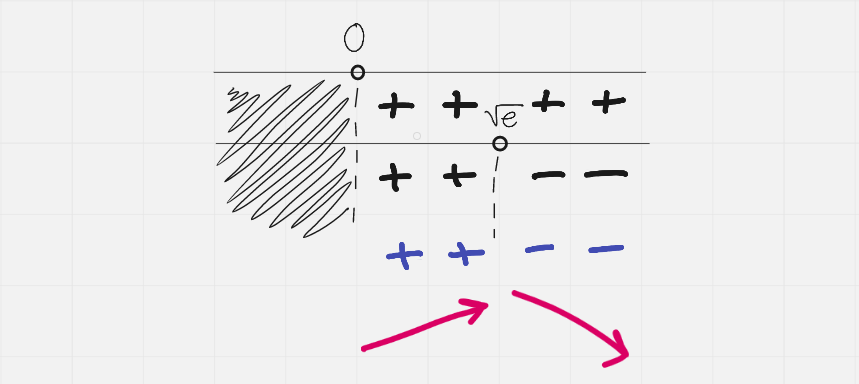
\includegraphics[width=\textwidth]{segno-luglio2021.png}
	studiando il segno noto che: $\sqrt{e}$ è punto di massimo assoluto.
	\paragraph*{5} Monotonia: Studiando il segno notiamo che la funzione è crescente in $(0,\sqrt{e})$ e decrescente in $[\sqrt{e},+\infty)$.
	\paragraph*{6} Punti di flesso: Studio la derivata seconda $f''(x)=\frac{2\ln(x)-3}{x^2}$.
	\\$f''(x)\geq 0$, $D>0 \forall x$,
	\\ $N\geq 0 \to \ln(x) \geq \frac{3}{2} \to x \geq e^{\frac{3}{2}}$.
	\\$e^{\frac{3}{2}}$ è un punto di flesso.
	\paragraph*{7} Tangente di flesso:
	\\$m = f'(e^{\frac{3}{2}}) = -\frac{2}{e^{\frac{3}{2}}}$
	\\$q = f(e^{\frac{3}{2}}) - f'(e^{\frac{3}{2}}) \cdot e^{\frac{3}{2}} = \frac{5}{4}$.
	\\Quindi la retta tangente ha equazione : $y=-\frac{2}{e^{\frac{3}{2}}} + \frac{5}{4}$.

}

\domandaaperta{2}{data la funzione $f(x)=x \sin x$
	\begin{enumerate}
		\item Si scrivano tutte le primitive
		\item Si determini,se esiste, la primitiva $\phi$ tale che $\phi(\pi) = 2\phi(0)$
		\item si calcoli $\int_{0}^{\pi} f(x) dx$
	\end{enumerate}
}
\rispostaaperta{
	\paragraph*{1} Integrando per parti (banale) trovo $F(x) = \sin x - \cos x + C$
	\paragraph*{3} $\int_{0}^{\pi} f(x) dx = F(\pi) - F(0) = \pi$
}


\chapter{Esercizi}
\section{Integrali}
\esercizio{}{
	$\int \frac{72}{\sqrt{x+49} + \sqrt{x+1}}$
}
\procedimento{
	Per questo esercizio bisogna fare un po di ragionamenti:
	\\Devo semplificare questa funzione, per fare ciò moltiplico e divido il tutto per la differenza del denominatore, quindi:
	$\int \frac{72}{\sqrt{x+49} + \sqrt{x+1}} \cdot \frac{\sqrt{x+49} - \sqrt{x+1}}{\sqrt{x+49} - \sqrt{x+1}}$
	\\Così ottengo : $\frac{3}{2}  \int (\sqrt{x+49} - \sqrt{x+1})$.
	\\A questo punto, posso separare gli integrali e risolverli singolarmente:
	$ = \frac{3}{2} \int (x+49)^{\frac{1}{2}} - \frac{3}{2} \int (x+1)^{\frac{1}{2}}$
}

\subsection{Esercitazione 10}
\esercizio{1}{$\int x^2 + 3x + 2 dx$}
\risposta{$\frac{2x^3+9x^2+12x}{6} + c$}
\procedimento{
	$\int x^2 + 3x + 2 dx = \int x^2 dx + 3\int x dx + 2 \int dx  = \frac{x^3}{3} + \frac{3x^2}{2} + 2x + c = ...$
}

\chapter{Cheatsheet}
\section*{Serie}
\paragraph*{Serie Armonica Generalizzata}
\begin{equation*}
	\sum \frac{1}{n^\alpha} \begin{cases}
		\text{Diverge}  & \alpha\leq 1 \\
		\text{Converge} & \alpha> 1
	\end{cases}
\end{equation*}
\paragraph*{Serie Geometrica}
\begin{equation*}
	\serie{0}{+\infty} q^n \begin{cases}
		\text{Diverge}    & q\geq 1 \\
		\text{Converge}   & -1<q<1  \\
		\text{Irregolare} & q\leq 1
	\end{cases}
\end{equation*}
\section*{Limiti}
\paragraph*{Ordine degli infiniti}
Nel calcolo dei limiti, quando bisogna trovare l'infinito di ordine maggiore:
$$ \log_ax\ll x^b\ll x^c\ll d^x\ll g^x\ll x^x $$
con $a>0 \wedge a\neq 1$, $0<b<c$, $1<d<g$
\nb{la radice è "più grande" del logaritmo}
\end{document}